\documentclass{article}
\usepackage[top=1in,bottom=1in]{geometry}
\usepackage{hyperref}
\usepackage{amssymb}
\usepackage{graphicx}
\graphicspath{ {./assets/} }
\usepackage[none]{hyphenat}
\usepackage{amsmath}
\date{}
\title{CMSC452 Elementary Theory of Computation}
\begin{document} 
  \author{Michael Li}
  \title{CMSC452 Elementary Theory of Computation}
  \maketitle
  \tableofcontents
  \newpage
  \section{Deterministic Finite Automata (DFA)}
  \subsection{Alphabet and Strings}
  $\Sigma$ is defined as the alphabet (e.g. $\{0, 1, 2\}$) and a \textbf{string} is a sequence of symbols of $\Sigma$ \\ \\
  $\Sigma^i = \{\sigma_1 \cdots \sigma_i \mid \sigma_1, \cdots, \sigma_i \in \Sigma \}$ \\ \\
  $\Sigma^0 = \{e\}$ the \textbf{empty string}. Useful for $w \cdot e = w$ (concatenation on string $w$) \\ \\
  $\Sigma^* = \Sigma^0 \cup \Sigma^1 \cup \cdots$ set of all strings including $e$ 
  \subsection{Concatenation, Number of a's, Prefix}
  Let $x, y \in \Sigma^*$. \textbf{Concatenation} of $x$ and $y$ is denoted $xy$ or $x \cdot y$. \\ \\
  If $A, B \subseteq \Sigma^*$ then $A \cdot B = \{ x \cdot y \mid x \in A \wedge y \in B\}$ \\ \\
  if $x \in \{a, b\}^*$ then $\#_a(x)$ is the number of $a$'s in $x$ \\ \\
  if $x \in \{a, b\}^*$ then $x \preceq y$ means that $x$ is a prefix of $y$
  \subsection{Modular Arithmetic}
  $x \equiv y \pmod{n}$ iff $n$ divides $x - y$
  \begin{itemize}
    \item Addition: wrap around $n$
    \item Multiplication: wrap around $n$
    \item Division: find a number $y$ such that $\frac{1}{x} * y \equiv 1 \pmod{n}$ \\ \\
      Example: $\frac{1}{3} \equiv 9\pmod{26}$ since $9 * 3 \equiv 1 \pmod{26}$ \\ \\
      \textbf{Note}: a number $x$ only has an inverse$\pmod n$ if $x$ and $n$ have no common factors
  \end{itemize}
  \subsection{DFA Formal Definition}
  \textbf{DFA} is a tuple $(Q, \Sigma, \delta, s, f)$ where
  \begin{itemize}
    \item $Q$ is a finite set of \textbf{state}
    \item $\Sigma$ is a finite alphabet
    \item $\delta \colon Q \times \Sigma \rightarrow Q$ is the \textbf{transition function}
    \item $s \in Q$ is the \textbf{start state}
    \item $F \subseteq Q$ is the set of \textbf{final states}
  \end{itemize}
  If $M$ is a DFA and $x \in \Sigma^*$, $M(x)$ \textbf{accepts} $x$ if when running $x$ through $m$ ends up in a final state. \\ \\
  The Language $L(M) = \{x \mid M(x) \text{ accepts}\}$ \\ \\
  Let $L \subseteq \Sigma^*$. If there exists a DFA $M$ such that $L(M) = L$ then $L$ is \textbf{regular} \\ \\
  DFA Limitations:
  \begin{itemize}
    \item DFA can only read 1 letter at a time and can never look at it again (one scan)
    \item DFA only has a finite number of states, $O(1)$ memory
    \item  DFA CAN keep track of $\#_a(w) \pmod{17}$
    \item DFA CANNOT keep track of $\#_a(w)$
  \end{itemize}
  \subsection{DFA Representations}
  \textbf{Normal DFA} that \textbf{accepts} and \textbf{rejecs} strings
    \begin{center}
      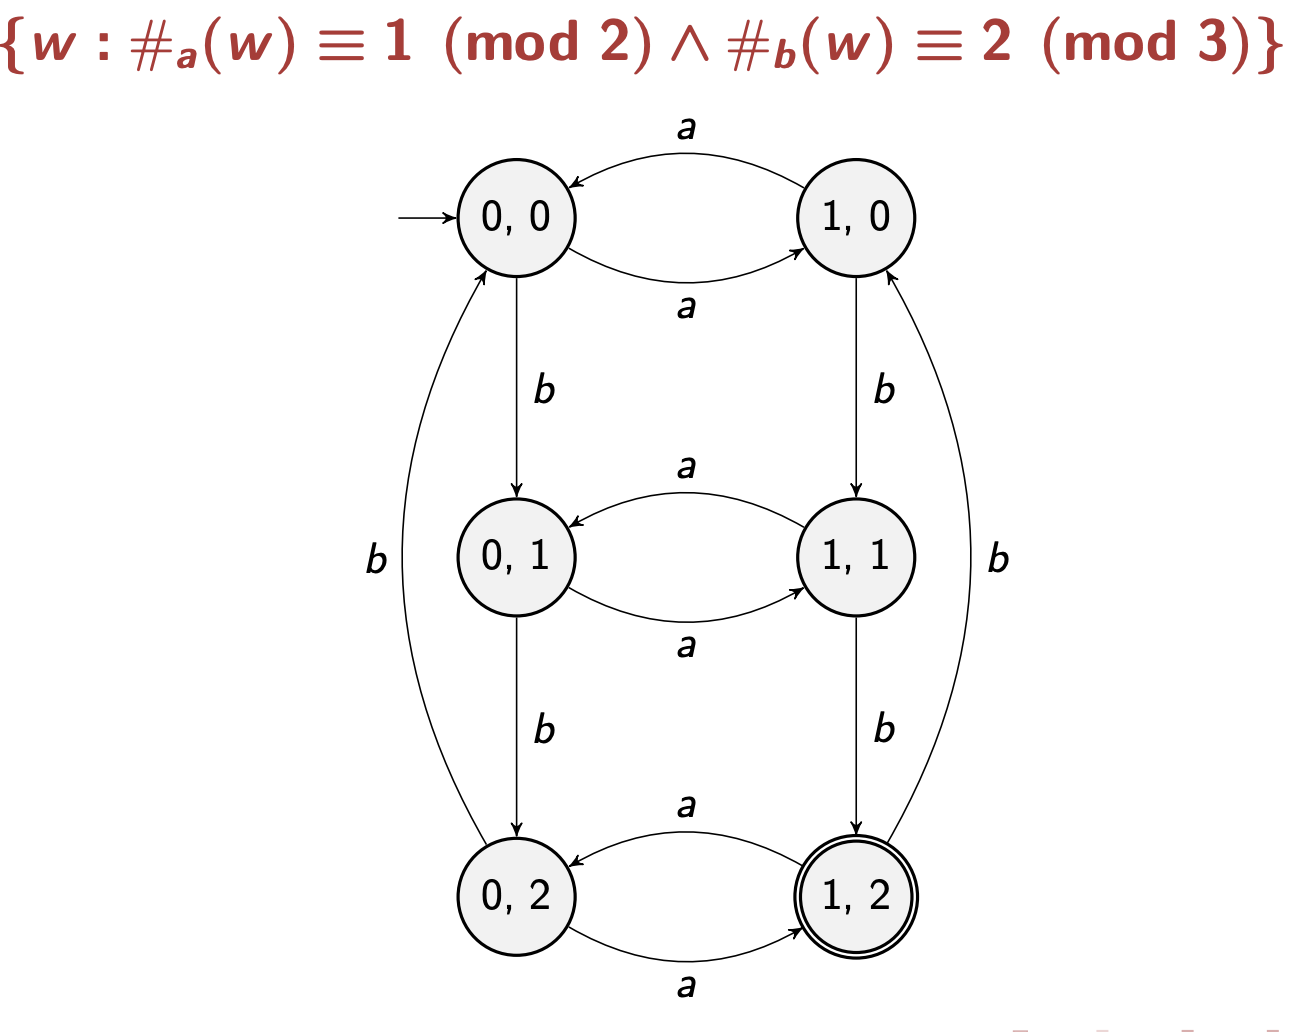
\includegraphics[scale=0.4]{normalDFA}
    \end{center}
    \textbf{DFA Classifer} that DOES NOT \textbf{accept} or \textbf{reject} strings. It \textbf{classifies} possible states.
  \begin{center}
    \includegraphics[scale=0.4]{DFACLassifier}
  \end{center}
  \textbf{Proof} the above DFA has at least 6 states. \\ \\
  Proof by contradiction: assume DFA $M$ has $\leq 5$ states.
  \begin{itemize}
    \item on input $e$, the empty string, goes to state $q_e$
    \item on input $a$, goes to state $q_a$
    \item on input $b$, goes to state $q_b$
    \item on input $bb$, goes to state $q_{bb}$
    \item on input $ab$, goes to state $q_{ab}$
    \item on input $abb$, goes to state $q_{abb}$
    \item Since $\leq 5$ states, 2 of these go to the same state (e.g. $q_{aa}$ and $a_{bb}$). However,
      \begin{itemize}
        \item $aa \cdot abb$ goes to some state $q_i$ which must accept since $aaabb \in L$
        \item $bb \cdot abb$ goes to some state $q_i$ which also must be accepted but $bbabb \notin L$. Thus, contradiction is reached.
        \item Would need to repeat the above contradiction for all pairs of $q$
      \end{itemize}
  \end{itemize} \\ \\
  \textbf{Transition Table Representation}
  \begin{center}
    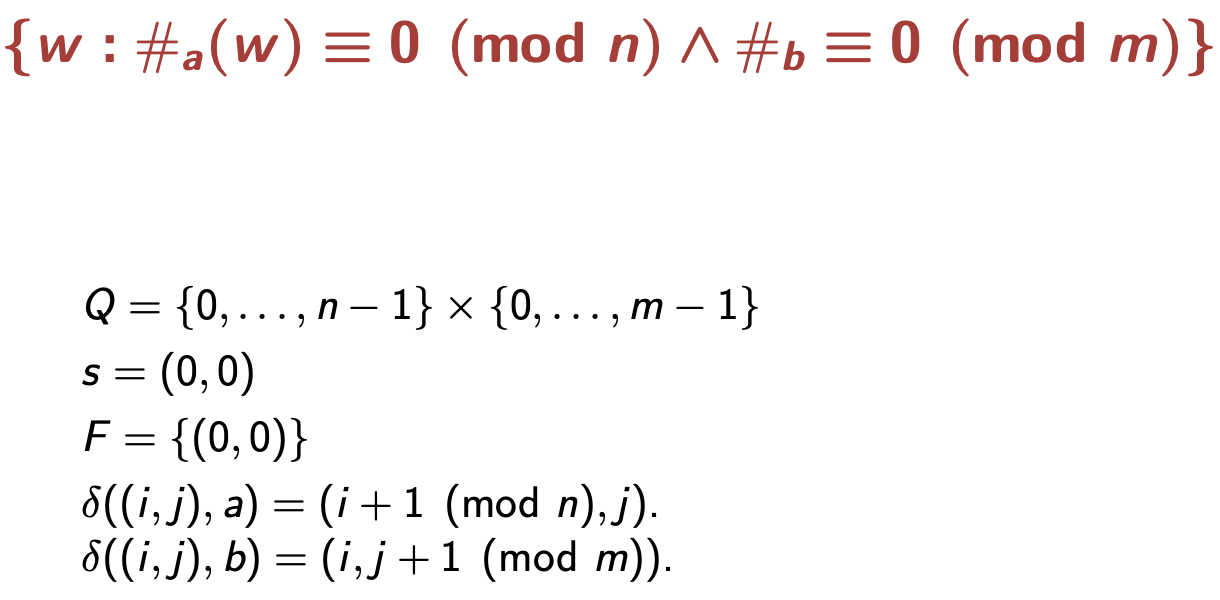
\includegraphics[scale=0.5]{TransitionTable}
  \end{center}
  Transition table will have $nm$ states \\ \\
  \textbf{Further Notes}: 
  \begin{itemize}
    \item For an alphabet $\Sigma = \{a, b\}$, $\Sigma^* a \Sigma^i$ can be done with $2^{i+1}$ states.
    \item Any finite set can be recognized by a DFA. Just draw a different state for each string in the set. This will take up around $2^n$ states, but typically can do this in fewer states. \\ \\
  \end{itemize}


\end{document}
